\section{Reference generation}
There are two ways for the user to interact with the multicopters: With a two joystick remote control (RC) or by sending various commands from the ground station PC.
For each approach we need to generate reasonable reference values $(\rR, \RR, \vR, \wR, \vRd, \wRd)[k]$ for the multicopter controller.

\paragraph{Euler angles and flat output.}
For the vast majority of multicopter maneuvers it is tilted less than $45^\circ$, so a minimal parameterization with singularities outside this working domain is tolerable.
A very popular parameterization for the rigid body attitude are the Euler angles in the roll-pitch-yaw convention $\tuple{\varepsilon} = [\rol, \pit, \yaw]^\top$:
\begin{align}\label{eq:RealizationEulerAngles}
 \R(\tuple{\varepsilon}) \!=\!
 \begin{bmatrix}
  \cyaw \cpit & -\syaw \crol+\cyaw \spit \srol & \syaw \srol+\cyaw \spit \crol \\
  \syaw \cpit & \cyaw \crol+\syaw \spit \srol & -\cyaw \srol+\syaw \spit \crol \\
  -\spit & \cpit \srol & \cpit \crol  
 \end{bmatrix}\!,
\quad
 \w(\tuple{\varepsilon}, \dot{\tuple{\varepsilon}}) \!=\!
 \begin{bmatrix} 
  \rold - \spit \yawd \\
  \cpit \srol \yawd + \crol \pitd\\
  \cpit \crol \yawd - \srol \pitd
 \end{bmatrix}
\end{align}
previously discussed in \autoref{sec:MotivationRigidBodyAttitude}.

As the tricopter is fully actuated, any minimal parameterization of its configuration space is a flat output.
One such parametrization is $\tuple{y} = (\rx, \ry, \rz, \rol, \pit, \yaw)$.

For the quadcopter, flatness was already discussed in \autoref{sec:CtrlExampleQuadcopter}. 
A reasonable flat output is $\tuple{y} = (\rx, \ry, \rz, \yaw)$.
The remainder of the attitude is then computed from the translational dynamics as
\begin{align}\label{eq:RealizationQuatFlatness}
 \Rz = \frac{\rdd - \gravityAcc}{\norm{\rdd - \gravityAcc}},
\qquad
 \rol = \arcsin(\cyaw \Ryz - \syaw\Rxz),
\quad
 \pit = \atanTwo(\cyaw\Rxz + \syaw \Ryz, \Rzz).
\end{align}
From these relations its clear that a feasible reference trajectory $t\mapsto \rR(t)$ for the position must be 4 times differentiable in order to compute the reference trajectory $t\mapsto\wRd(t)$ for the angular acceleration.
The singularity for $\rdd = \gravityAcc$, is practically not realizable, since the propellers have a minimum thrust, i.e.\ free fall is not feasible.


\paragraph{Real-time trajectory generator.}
The multicopter firmware includes a real-time trajectory generaor for the corresponding flat output discussed above.
It knows the current reference $\tuple{y}_\idxRef(t), \ldots, \tuple{y}^{(4)}_\idxRef(t)$ and when receiving a new static setpoint $\tuple{y}_\idxRef(t+T) = \const$, with a given transition time $T$, it computes and evaluates the interpolating polynomials of sufficient degree.
The actutual reference values $(\rR, \RR, \vR, \wR, \vRd, \wRd)[k]$ for the main rigid body controller are computed from \eqref{eq:RealizationQuatFlatness}, \eqref{eq:RealizationEulerAngles} and their derivatives.

The setpoints are the standard command interface for the multicopter GUI on the groundstation PC.
The results in \autoref{fig:TriManeuver42Result} and \autoref{fig:QuadManeuver42Result} which are discussed in the next section utilized these trajectories.

\paragraph{Precomputed position trajectories.}
For specific maneuvers its also possible to execute a precomputed, sampled position trajectory $k \mapsto \rR[k]$ stored on the multicopter controller.
For the tricopter, the attitude is hold constant during the maneuver.
This mode was used for the experimental results in \cite{Irscheid:HeavyRopesTricopter}.

Analog to this, for the quadcopter, we could hold the yaw angle constant.
However, this mode is used for aerobatic maneuvers where the singularities of the Euler angles are unacceptable.
Also, as discussed in \cite{Konz:QuadrotorMovingFrame}, the hairy ball theorem \cite{Brouwer:HairyBallTheorem} implies that any flat output of the quadcopter model must have a singularity somewhere.
On the other hand, we usually do not care to much about the actual heading of the copter, but only want it to be somewhat steady about this degree of freedom.

So instead of parameterizing the heading we use the angular velocity $\wRz$ and \textit{integrate} the remaining attitude from:
\begin{subequations}
\begin{align}
 \RRz &= \frac{\rRdd - \gravityAcc}{\norm{\rRdd - \gravityAcc}},&
 \RRzd &= \frac{\rRddd - \sProd{\rRddd}{\RRz} \RRz}{\norm{\rRdd - \gravityAcc}},
\\
 \RRxd &= \wRz \RRy - \wRy \RRz,&
 \wRy &= \RRx^\top \RRzd
\\
 \RRyd &= \wRx \RRz - \wRz \RRx,&
 \wRx &= -\RRy^\top \RRzd.
\end{align}
\end{subequations}
This trajectory generation mode with $\wRz=0$ was used for the quadcopter looping (\autoref{fig:QuadLoopResult}) and the quadcopter flip experiment (\autoref{fig:QuadFlipResult}).


\paragraph{Remote control mode.}
In this mode the position measurements are not available or not used, e.g.\ in outdoor experiments.
Instead a human pilot is tasked with controlling the multicopter with a two joystick remote control (RC).

The parameters of the rigid body controller, see \autoref{chap:Ctrl}, are set as follows:
The desired ineria coincides with the model inertia, i.e.\ $\mc = m, \Jc = \J, \sc=\tuple{0}$.
The center of damping and stiffness coincides with the center of mass $\lc=\hc=\tuple{0}$.
As previously discused in \autoref{sec:DecouplingRigidBody}, this decouples the rotational part of the closed loop dynamics.
As the pilot is charged with controlling th position, we set vanishing translational stiffness $\kc=0$ and damping $\dc=0$.
For the particle based approach (see \autoref{sec:CtrlApproachParticlesSingleBody}) this results in the trivial closed loop dynamics $\rdd = \rRdd$ andthe translational part of the explicit control law reads
\begin{align}\label{eq:RealizationPilotTranslationControl}
 \bodyForce{}{} = m \R^\top (\rRdd - \gravityAcc)
\end{align}
Unfortunatly, for the body-based and energy based approaches, terms with $\r-\rR$ and $\rd-\rRd$ still appear in gyroscopic terms.
For the actual microcontroller implementation these terms were simply set to zero which ultimatly implies the same translational control as for the particle based approach \eqref{eq:RealizationPilotTranslationControl}.

In practice, the forward direction of the multicopter is more intuitive to a pilot than the e.g.\ the north directions.
With similar arguments \cite{Kastelan:Tricopter} proposes the use of a heading referenced acceleration $\tuple{a}_\idxRef = \R_{\mathsf{Z}}^\top(\yaw_\idxRef) \rRdd$ which is used in the following as well.
Furthermore, its practical to set the yaw rate $\dot{\yaw}_\idxRef$ and integrate the angle within the controller.
Overall, the analog channels of the RC are associated with the the reference quantities $(a_{\mathsf{x}\idxRef}, a_{\mathsf{y}\idxRef}, a_{\mathsf{z}\idxRef}, \rol_\idxRef, \pit_\idxRef, \dot{\yaw}_\idxRef)$ for the tricopter and $(a_{\mathsf{x}\idxRef}, a_{\mathsf{y}\idxRef}, a_{\mathsf{z}\idxRef}, \dot{\yaw}_\idxRef)$ for the quadcopter.

\begin{figure}
\centering
%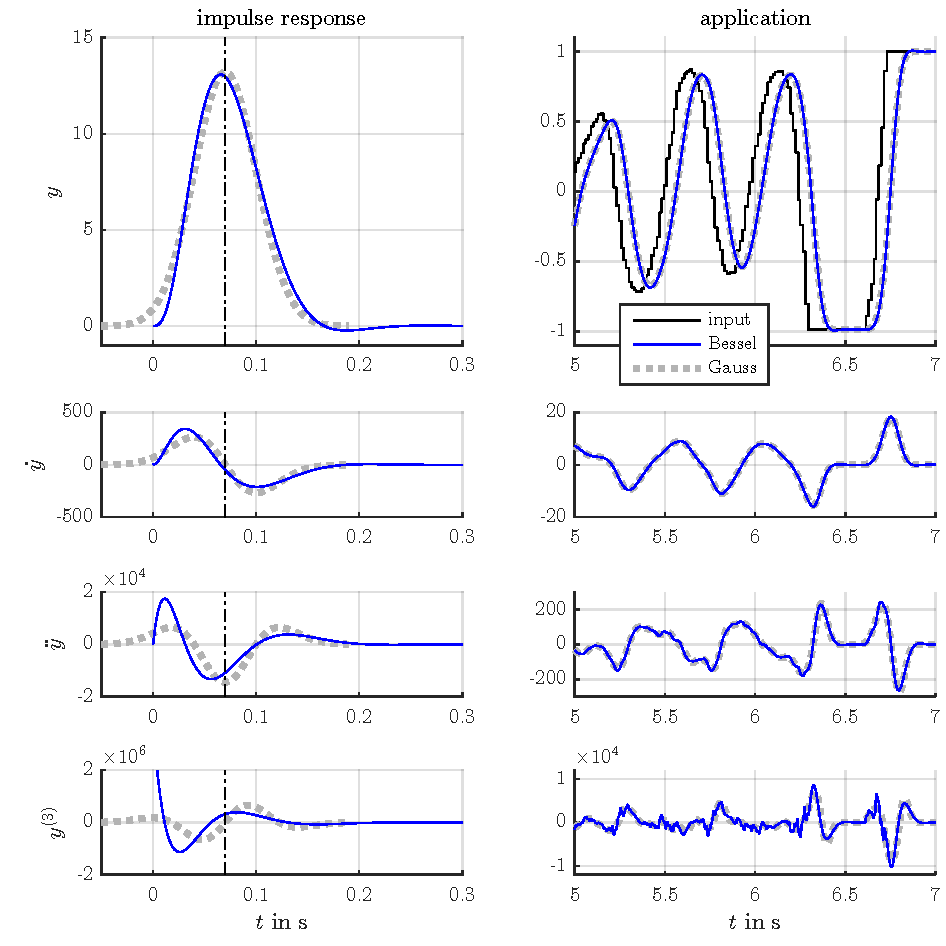
\includegraphics{RCFilter/RCFilter.pdf} 
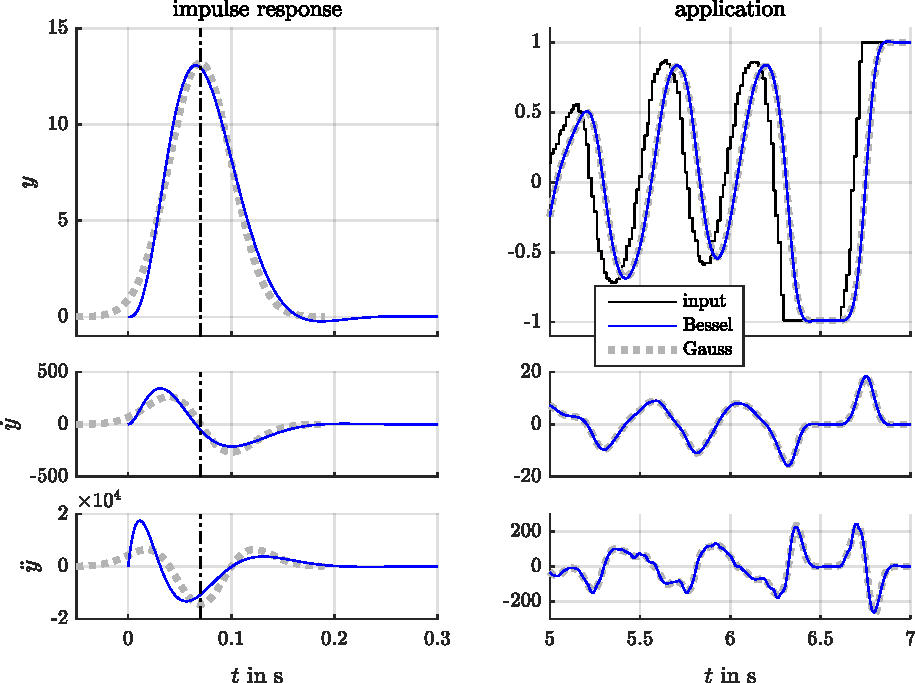
\includegraphics{RCFilter/RCFilterMod.pdf} 
\caption{Application of the filter to the RC input}
\label{fig:RCFilter}
\end{figure}

In order to smoothen the RC signals $\uRC$ and obtain the required derivatives at the same time we utilize a simple low pass filter
\begin{align}\label{eq:RealizationRCFilter}
 \tdiff{t} \begin{bmatrix} \yRC[] \\ \yRCd[] \\ \yRCdd[] \\ \yRCddd[] \end{bmatrix}
 &= \begin{bmatrix} 0 & 1 & 0 & 0 \\ 0 & 0 & 1 & 0 \\ 0 & 0 & 0 & 1 \\ -a_0 & -a_1 & -a_2 & -a_3 \end{bmatrix}
 \begin{bmatrix} \yRC[] \\ \yRCd[] \\ \yRCdd[] \\ \yRCddd[] \end{bmatrix}
 + \begin{bmatrix} 0 \\ 0 \\ 0 \\ a_0 \end{bmatrix}
 \uRC[]
\end{align}
The filter coefficients $a_i$ are chosen to resemble a (continuous) Bessel filter with cutoff frequency $7\,\unit{Hz}$, see e.g.\ \cite[sec.\,13.1.3]{TietzeSchenk:Halbleiter-Schaltungstechnik}.
A Bessel filter is characterized by having a maximally flat group delay, i.e.\ it preserves the (time-domain) shape of the signal in the passband (opposed to a Butterworth filter which preserves the amplitude in the frequency domain).
With rising order the (IIR) Bessel filter converges to a (FIR) Gaussian filter \cite[sec.\ 4.9.2]{Rabiner:DSP}.

The actual implementation is the exaxt discretization of \eqref{eq:RealizationRCFilter}.
\autoref{fig:RCFilter} shows the impulse response and application to a measured example RC-channel of the used Bessel filter and a corresponding Gaussian filter (windowlength 43).
Even though the difference is visible on the impulse response, the result of the implemented filter and the Gauss filter are indistinguishable in the practical application.

